%% LaTeX-Beamer template for KIT design
%% by Erik Burger, Christian Hammer
%% title picture by Klaus Krogmann
%%
%% version 2.1
%%
%% mostly compatible to KIT corporate design v2.0
%% http://intranet.kit.edu/gestaltungsrichtlinien.php
%%
%% Problems, bugs and comments to
%% burger@kit.edu

\documentclass[18pt]{beamer}

%% SLIDE FORMAT

% use 'beamerthemekit' for standard 4:3 ratio
% for widescreen slides (16:9), use 'beamerthemekitwide'

\usepackage{templates/beamerthemekit}
\usepackage[utf8]{inputenc}
\usepackage[T1]{fontenc}
\usepackage{graphicx}
\usepackage{tikz}

% \usepackage{templates/beamerthemekitwide}

%% TITLE PICTURE

% if a custom picture is to be used on the title page, copy it into the 'logos'
% directory, in the line below, replace 'mypicture' with the 
% filename (without extension) and uncomment the following line
% (picture proportions: 63 : 20 for standard, 169 : 40 for wide
% *.eps format if you use latex+dvips+ps2pdf, 
% *.jpg/*.png/*.pdf if you use pdflatex)

\titleimage{sheep}

%% TITLE LOGO

% for a custom logo on the front page, copy your file into the 'logos'
% directory, insert the filename in the line below and uncomment it

%\titlelogo{mylogo}

% (*.eps format if you use latex+dvips+ps2pdf,
% *.jpg/*.png/*.pdf if you use pdflatex)

%% TikZ INTEGRATION

% use these packages for PCM symbols and UML classes
% \usepackage{templates/tikzkit}
% \usepackage{templates/tikzuml}

% the presentation starts here

\title{Zwischenpräsentation der Java-Gruppe}
\subtitle{Neuronale Netze mit Neuroph}
\author{Markus Braun, Daniel Hammann, Dominik Messinger, Dominic Rausch}

\institute{Institut für Programmstrukturen und Datenorganisation (IPD), Lehrstuhl für Programmiersysteme}

% Bibliography

%\usepackage[citestyle=authoryear,bibstyle=numeric,hyperref,backend=biber]{biblatex}
%\addbibresource{templates/example.bib}
%\bibhang1em

\begin{document}
	\maketitle

	\begin{frame}[c]\frametitle{Neuronale Netze}
		\begin{block}{Einleitung}
		    \begin{itemize}
			    \item Bestehen aus Neuronen (Verarbeitungseinheiten)
		    	\item Gewichtete Eingabeverbindungen werden zusammenfasst (Propagierungsfunktion)
		    	\item Aktivierungsfunktion mit Schwellwert
		    	\item Aus Aktivierung folgt mittels Ausgabefunktion die Ausgabe
		    \end{itemize}		    
		\end{block}	
		\vspace{.5cm}
			\begin{minipage}[c]{0.48\textwidth}
				\begin{center}
				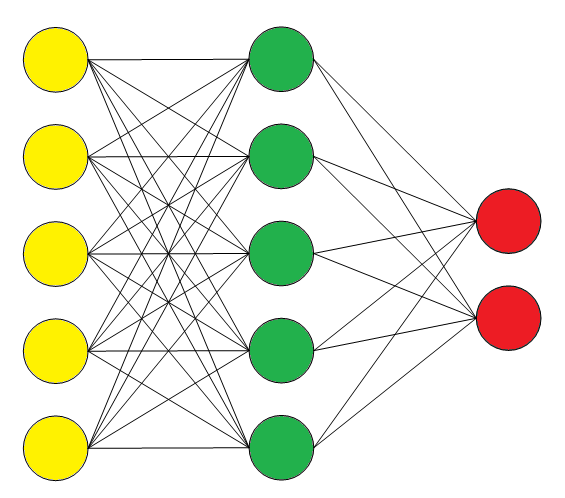
\includegraphics[width=0.5\textwidth]{images/ann.png}
				\end{center}
			\end{minipage}	
			\begin{minipage}[c]{0.48\textwidth}
				\begin{center}
				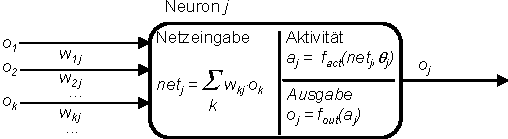
\includegraphics[width=\textwidth]{images/Neuron}
				\end{center}				
			\end{minipage}
\begin{flushright}
			\tiny{[Quelle: Lehr- und Übungsbuch künstliche Intelligenz; Lämmel, Cleve; 2012]}
\end{flushright}
	\end{frame}

	%!TEX root = abschlusspraesentation.tex

\begin{frame}[c]\frametitle{NN Auswertung}
\usetikzlibrary{arrows}
\usetikzlibrary{positioning} 
\usetikzlibrary{automata} 

  \def\wOne{{1.0,2.0,3.0,4.0}}
  \def\wTwo{{2.0,1.0,4.0,2.0,3.0,1.0}}

  \def\wOneAdjusted{{0.9,2.2,2.7,3.6}}
  \def\wTwoAdjusted{{3.0,0.5,3.7,1.8,2.5,0.5}}

  \def\inputValues{{0.3,0.2,0.5,0.6}}
  \def\results{{0.3,0.4,1.5,2.4}}
  \def\allresults{{-2.0, 4.6, 5.7, -3.0, 1.0, 4.4}}
  \def\allresultstransfered{{0.4, 0.8, 0.9, 0.3, 0.55, 0.8}}
  
  \def\rightresults{{0.3,0.4,1.5,2.4,2.0,2.0}}
  \def\allrightresults{{-5.7, 4.6, -5.7}}
  \def\allrightresultstransfered{{0.1, 0.8, 0.1}}
  \def\error{{-0.1, 0.2, -0.1}}
  \def\deltasoutput{{-0.0, 0.0, -0.0}}
  \def\deltashidden{{0.0, 0.0, 0.0, 0.0, 0.0, 0.0}}

  \begin{tikzpicture}[->,shorten >=1pt,auto, node distance=1cm, scale=0.9,
    thick,main node/.style={circle,fill=blue!20,draw,font=\sffamily\small\bfseries}]
    % =======
    % empty invisible node to avoid resize
    % =======
      \node at (-2,7) {};
    % =======
    % Input Neurons   
    % =======
    \only<1>{
      \foreach \x in {0, ..., 3} {
        \node[main node] (\x) at (0,5.8-1.2*\x) {};
      }
    }
    \only<2->{
      \foreach \x in {0, ..., 3} {
        \node[main node] (\x) at (0,5.8-1.2*\x) {$\pgfmathparse{\inputValues[\x}\pgfmathresult$};
      }
    }


    % =======
    % Hidden Neurons   
    % =======
    \only<1-3> {
      \foreach \x in {0, ..., 5} {
        \node[main node] (1\x) at (4,7-1.2*\x) {};
      }
    }
    \only<4> {
      \foreach \x in {0,2,3,4,5} {
        \node[main node] (1\x) at (4,7-1.2*\x) {};
      }
      \node[main node] (11) at (4,7-1.2) {$\pgfmathparse{\allresults[1}\pgfmathresult$};
    }
    \only<5> {
      \foreach \x in {0,...,5} {
        \node[main node] (1\x) at (4,7-1.2*\x) {$\pgfmathparse{\allresults[\x}\pgfmathresult$};
      }
    }
     \only<6-13> {
      \foreach \x in {0,...,5} {
        \node[main node] (1\x) at (4,7-1.2*\x) {$\pgfmathparse{\allresultstransfered[\x}\pgfmathresult$};
      }
    }
    \only<14-> {
      \foreach \x in {0,...,5} {
        \node[main node] (1\x) at (4,7-1.2*\x) {$\pgfmathparse{\deltashidden[\x}\pgfmathresult$};
      }
    }


    % =======
    % Output Neurons   
    % =======
    \only<1-7> {
      \foreach \x in {0, ..., 2} {
        \node[main node] (2\x) at (8,5.2-1.2*\x) {};
      }
    }
    \only<8> {
      \foreach \x in {0, 2} {
        \node[main node] (2\x) at (8,5.2-1.2*\x) {};
      }
       \node[main node] (21) at (8,5.2-1.2) {$\pgfmathparse{\allrightresults[1}\pgfmathresult$};
    }
     \only<9> {
      \foreach \x in {0,..., 2} {
        \node[main node] (2\x) at (8,5.2-1.2*\x) {$\pgfmathparse{\allrightresults[\x}\pgfmathresult$};
      }
       
    }
     \only<10> {
      \foreach \x in {0,..., 2} {
        \node[main node] (2\x) at (8,5.2-1.2*\x) {$\pgfmathparse{\allrightresultstransfered[\x}\pgfmathresult$};
      }
       
    }

    \only<11> {
      \foreach \x in {0,..., 2} {
          \node[main node] (2\x) at (8,5.2-1.2*\x) {$\pgfmathparse{\error[\x}\pgfmathresult$};
      }
    }
    \only<12-> {
      \foreach \x in {0,..., 2} {
          \node[main node] (2\x) at (8,5.2-1.2*\x) {$\pgfmathparse{\deltasoutput[\x}\pgfmathresult$};
      }
    }

    
    


    
    % \ifthenelse{\iStepTwo>0 \and \iStepTwo<11}{
    %   \foreach \x in {0, ..., 3} {
    %     \node at (0.1*\iStepTwo,5.8-1.2*\x+\iStepTwo*\x*0.06) {\pgfmathparse{\inputValues[\x}\pgfmathresult};
    %   }
    % } 

    % \ifthenelse{\iStepThree>0 \and \iStepThree<11}{
    %   \foreach \x in {0, ..., 3} {
    %     \node [opacity=1.0-0.1*\iStepThree] at (1.0+0.08*\iStepThree,5.8-0.6*\x) {\pgfmathparse{\inputValues[\x}\pgfmathresult};
    %   }
    % } 

    % \ifthenelse{\iStepFour>0 \and \iStepFour<11}{
    %   \foreach \x in {0, ..., 3} {
    %     \node [opacity=0.1*\iStepFour] at (1.8,5.8-0.6*\x) {\pgfmathparse{\results[\x}\pgfmathresult};
    %   }
    % } 

    % \ifthenelse{\iStepFive>0 \and \iStepFive<11}{
    %   \foreach \x in {0, ..., 3} {
    %     \node at (1.8+0.2*\iStepFive,5.8-0.6*\x+0.06*\iStepFive*\x) {\pgfmathparse{\results[\x}\pgfmathresult};
    %   }
    % } 
    
    % =======
    % edges   
    % ======= 
    \only<1> {
      \foreach \x in {0, ..., 3} 
        \foreach \y in {0, ..., 5} {
          \ifthenelse{\y=1}{
            \path[every node/.style={font=\sffamily\small}]
              (\x) edge [opacity=0.5] node [left] {} (1\y);
          }{
            \path[every node/.style={font=\sffamily\small}]
              (\x) edge [opacity=0.2] node [left] {} (1\y);
          }
        }
      
      \foreach \x in {0, ..., 5} 
        \foreach \y in {0, ..., 2} {
          \ifthenelse{\y=1}{
            \path[every node/.style={font=\sffamily\small}]
              (1\x) edge [opacity=0.5] node [left] {} (2\y);
          }{
            \path[every node/.style={font=\sffamily\small}]
              (1\x) edge [opacity=0.2] node [left] {} (2\y);
          }
        }
    }
    
    \only<2> {
      \foreach \x in {0, ..., 3} 
        \foreach \y in {0, ..., 5} {
          \ifthenelse{\y=1}{
            \path[every node/.style={font=\sffamily\small}]
              (\x) edge [opacity=0.5] node [left, sloped, above, opacity=1.0] {$\pgfmathparse{\wOne[\x}\pgfmathresult$} (1\y);
          }
        }
      
      \foreach \x in {0, ..., 5} 
        \foreach \y in {0, ..., 2} {
          \ifthenelse{\y=1}{
            \path[every node/.style={font=\sffamily\small}]
              (1\x) edge [opacity=0.5] node [left, sloped, above, opacity=1.0] {$\pgfmathparse{\wTwo[\x}\pgfmathresult$} (2\y);
          }
        }
    }

    \only<3> {
      \foreach \x in {0, ..., 3} 
        \foreach \y in {0, ..., 5} {
          \ifthenelse{\y=1}{
            \path[every node/.style={font=\sffamily\small}]
              (\x) edge [opacity=0.5] node [left, sloped, above, opacity=1.0, pos=0.4] {$\pgfmathparse{\inputValues[\x}\pgfmathresult\cdot\pgfmathparse{\wOne[\x}\pgfmathresult=\pgfmathparse{\results[\x}\pgfmathresult$} (1\y);
          }
        }
      
      \foreach \x in {0, ..., 5} 
        \foreach \y in {0, ..., 2} {
          \ifthenelse{\y=1}{
            \path[every node/.style={font=\sffamily\small}]
              (1\x) edge [opacity=0.5] node [left, sloped, above, opacity=1.0] {$\pgfmathparse{\wTwo[\x}\pgfmathresult$} (2\y);
          }
        }
    }

    \only<4-6> {
      \foreach \x in {0, ..., 3} 
        \foreach \y in {0, ..., 5} {
          \ifthenelse{\y=1}{
            \path[every node/.style={font=\sffamily\small}]
              (\x) edge [opacity=0.5] node [left, sloped, above, opacity=1.0, pos=0.4] {$\pgfmathparse{\wOne[\x}\pgfmathresult$} (1\y);
          }
        }
      
      \foreach \x in {0, ..., 5} 
        \foreach \y in {0, ..., 2} {
          \ifthenelse{\y=1}{
            \path[every node/.style={font=\sffamily\small}]
              (1\x) edge [opacity=0.5] node [left, sloped, above, opacity=1.0] {$\pgfmathparse{\wTwo[\x}\pgfmathresult$} (2\y);
          }
        }
    }
    \only<7> {
      \foreach \x in {0, ..., 3} 
        \foreach \y in {0, ..., 5} {
          \ifthenelse{\y=1}{
            \path[every node/.style={font=\sffamily\small}]
              (\x) edge [opacity=0.5] node [left, sloped, above, opacity=1.0, pos=0.4] {$\pgfmathparse{\wOne[\x}\pgfmathresult$} (1\y);
          }
        }
      
      \foreach \x in {0, ..., 5} 
        \foreach \y in {0, ..., 2} {
          \ifthenelse{\y=1}{
            \path[every node/.style={font=\sffamily\small}]
              (1\x) edge [opacity=0.5] node [left, sloped, above, opacity=1.0, pos=0.4] {$\pgfmathparse{\allresultstransfered[\x}\pgfmathresult\cdot\pgfmathparse{\wTwo[\x}\pgfmathresult=\pgfmathparse{\rightresults[\x}\pgfmathresult$} (2\y);
          }
        }
    }
    \only<8-12> {
      \foreach \x in {0, ..., 3} 
        \foreach \y in {0, ..., 5} {
          \ifthenelse{\y=1}{
            \path[every node/.style={font=\sffamily\small}]
              (\x) edge [opacity=0.5] node [left, sloped, above, opacity=1.0, pos=0.4] {$\pgfmathparse{\wOne[\x}\pgfmathresult$} (1\y);
          }
        }
      
      \foreach \x in {0, ..., 5} 
        \foreach \y in {0, ..., 2} {
          \ifthenelse{\y=1}{
            \path[every node/.style={font=\sffamily\small}]
              (1\x) edge [opacity=0.5] node [left, sloped, above, opacity=1.0] {$\pgfmathparse{\wTwo[\x}\pgfmathresult$} (2\y);
          }
        }
    }
    \only<13-14> {
      \foreach \x in {0, ..., 3} 
        \foreach \y in {0, ..., 5} {
          \ifthenelse{\y=1}{
            \path[every node/.style={font=\sffamily\small}]
              (\x) edge [opacity=0.5] node [left, sloped, above, opacity=1.0, pos=0.4] {$\pgfmathparse{\wOne[\x}\pgfmathresult$} (1\y);
          }
        }
      
      \foreach \x in {0, ..., 5} 
        \foreach \y in {0, ..., 2} {
          \ifthenelse{\y=1}{
            \path[every node/.style={font=\sffamily\small}]
              (1\x) edge [opacity=0.5] node [left, sloped, above, opacity=1.0] {$\pgfmathparse{\wTwoAdjusted[\x}\pgfmathresult$} (2\y);
          }
        }
    }
    \only<15-> {
      \foreach \x in {0, ..., 3} 
        \foreach \y in {0, ..., 5} {
          \ifthenelse{\y=1}{
            \path[every node/.style={font=\sffamily\small}]
              (\x) edge [opacity=0.5] node [left, sloped, above, opacity=1.0, pos=0.4] {$\pgfmathparse{\wOneAdjusted[\x}\pgfmathresult$} (1\y);
          }
        }
      
      \foreach \x in {0, ..., 5} 
        \foreach \y in {0, ..., 2} {
          \ifthenelse{\y=1}{
            \path[every node/.style={font=\sffamily\small}]
              (1\x) edge [opacity=0.5] node [left, sloped, above, opacity=1.0] {$\pgfmathparse{\wTwoAdjusted[\x}\pgfmathresult$} (2\y);
          }
        }
    }
   \end{tikzpicture}
  \begin{itemize}
    \only<1> {
      \item Multilayerperceptron-Netz
    }
    \only<2> {
      \item Trainingseingabe und Kantengewichte
    }
    \only<3> {
      \item Gewichtung der Trainingseingabe mit Kantengewicht
    }
    \only<4> {
      \item Summe der Produkte ergibt Netzeingabe in der Hidden-Schicht
    }
    \only<5> {
      \item Netzeingabe der restlichen Neuronen der Hidden-Schicht
    }
    \only<6> {
      \item Umrechnung der Netzeingabe mit der Übertragungsfunktion (sigmoiddelta)
    }
    \only<7> {
      \item Gewichtung der Ausgabewerte mit Kantengewicht
    }
    \only<8> {
      \item Summe der Produkte ergibt Netzeingabe in der Ausgabeschicht
    }
    \only<9> {
      \item Netzeingabe der restlichen Neuronen der Ausgabeschicht
    }
    \only<10> {
      \item Umrechnung der Netzeingabe mit der Übertragungsfunktion (sigmoiddelta)
    }
    \only<11> {
      \item Berechnung des Ausgabefehlers anhand Ausgabewert und gewünschtem Ausgabewert
    }
    \only<12> {
      \item Berechnung von delta-Werten anhand Netzeingabe, Übertragungsfunktion und Ausgabefehler 
    }
    \only<13> {
      \item Anpassung der Kantengewichte
    }
    \only<14> {
      \item Berechnung von delta-Werten in Hidden-Schicht (benötigt u.a. ausgehende Kantengewichte und delta-Werte der Ausgabeschicht)
    }
    \only<15> {
      \item Anpassung der Kantengewichte
    }
   \end{itemize}
  
% \item<1> Multilayerperceptron-Netz
%       \item<2> Trainingseingabe und Kantengewichte
%       \item<3> Gewichtung der Trainingseingabe mit Kantengewicht
%       \item<4> Summe der Produkte ergibt Netzeingabe in der Hidden-Schicht
%       \item<5> Netzeingabe der restlichen Neuronen der Hidden-Schicht
%       \item<6> Umrechnung der Netzeingabe mit der Übertragungsfunktion (sigmoiddelta)
%       \item<7> Gewichtung der Ausgabewerte mit Kantengewicht
%       \item<8> Summe der Produkte ergibt Netzeingabe in der Output-Schicht
%       \item<9> Netzeingabe der restlichen Neuronen der Output-Schicht
%       \item<10> Umrechnung der Netzeingabe mit der Übertragungsfunktion (sigmoiddelta)
%       \item<11> b
%       \item<12> Berechnung von delta-Werten anhand Netzeingabe, Übertragungsfunktion und Ausgabefehler 
%       \item<13> b

    % \node[main node] (0) {5};
    % \node[main node] (1) [below of=0] {\only<2>{test}};
    % \node[main node] (2) [below of=1] {3};
    % \node[main node] (3) [below of=2] {4};

    % \node[main node] (11) [right of=0] {2};
    % \node[main node] (10) [above of=11] {2};
    % \node[main node] (12) [right of=1] {2};
    % \node[main node] (13) [right of=2] {2};
    % \node[main node] (14) [right of=3] {2};
    % \node[main node] (15) [below of=14] {2};

    % \node[main node] (20) [below right  of=10] {2};
    % \node[main node] (21) [below right  of=12] {2};
    % \node[main node] (22) [below right  of=14] {2};

    % \path[every node/.style={font=\sffamily\small}]
    %   (0) edge node [left] {0.6} (10)
    %       edge node[left] {0.3} (11)
    %       edge node {0.1} (12)
    %   (1) edge node [right] {0.4} (10)
    %       edge node {0.3} (11)
    %       edge node {0.4} (12)
    %       edge node {0.1} (13)
    %   (2) edge node [right] {0.8} (13)
    %       edge node [right] {0.2} (14)
    %       edge node [right] {0.2} (15)
    %   (3) edge node [left] {0.2} (15)

    %   (10)edge node [left] {0.6} (20)
    %   (11)edge node [right] {0.4} (20)
    %       edge node {0.3} (21)
    %       edge node {0.4} (22)
    %   (12)edge node [right] {0.8} (21)
    %       edge node [right] {0.2} (20)
    %   (13)edge node [left] {0.2} (20)
    %   (14)edge node [right] {0.8} (21)
    %       edge node [right] {0.2} (22)
    %   ;
    
\end{frame}
	

	\begin{frame}[c]\frametitle{Neuronale Netze}
		\begin{center}
		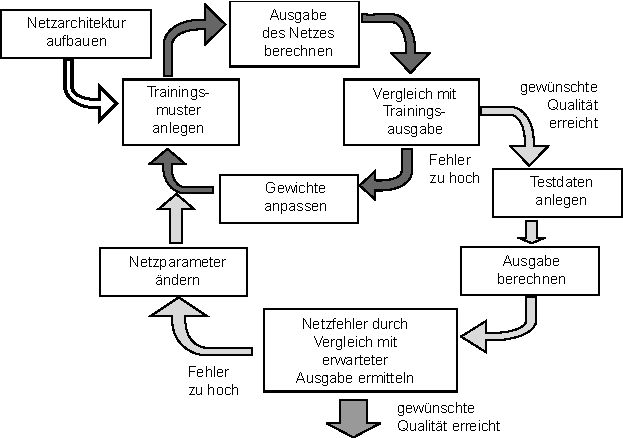
\includegraphics[scale=.8]{images/workflow}
		\end{center}
		\begin{flushright}
		\tiny{[Quelle: Lehr- und Übungsbuch künstliche Intelligenz; Lämmel, Cleve; 2012]}
		\end{flushright}
	\end{frame}		

	\begin{frame}[c]\frametitle{Überblick}
		\begin{block}{Was bisher geschah}
		    \begin{itemize}
		    	\item Einarbeitung in die Thematik der Neuronale Netze
			    \item Testdaten beschaffen
		    	\item Code Analyse der Simulationsumgebung Neuroph
		    	\item Drei Parallelisierungsversuche
		    	\item Profiling (u.a. eigenes Evaluierungsframework)
		    \end{itemize}		    
		\end{block}
	\end{frame}
	
	\begin{frame}[c]\frametitle{Testdaten}
		\begin{block}{Erste Versuche}
		    \begin{itemize}
		    	\item StockExchange - Börsenvorhersage
		    	\item IrisScan Datensatz
		    \end{itemize}
		\end{block}
		\begin{block}{Teilchenkollision (Cern)}
		    \begin{itemize}
		    	\item 15k Datensätze
		    	\item Eingabe: 2853 Sensorwerte
				\item Ausgabe: Ist das Ereignis interessant oder nicht? 
				%Schwarzes Loch oder nicht?
		    \end{itemize}
		\end{block}		
	\end{frame}

	\begin{frame}[c]\frametitle{Code Analyse \& Profiling}
		\begin{block}{Was wir vorgefunden haben}
			\begin{center}
				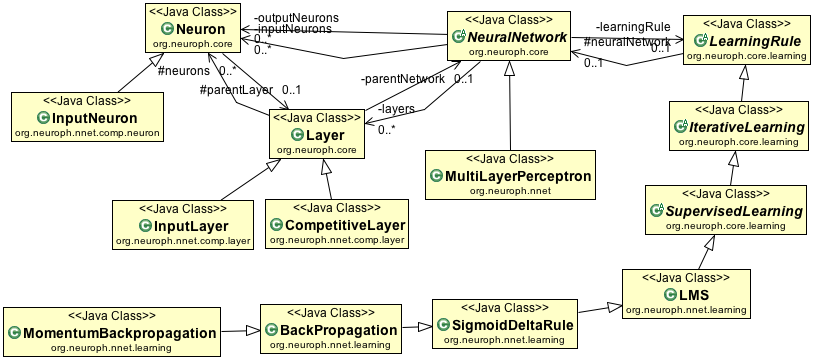
\includegraphics[scale=0.4]{images/Klassendiagramm.png}
			\end{center}
		\end{block}
	\end{frame}
	
	\begin{frame}[c]\frametitle{Code Analyse: Sequenzdiagramm}
			\begin{center}
			  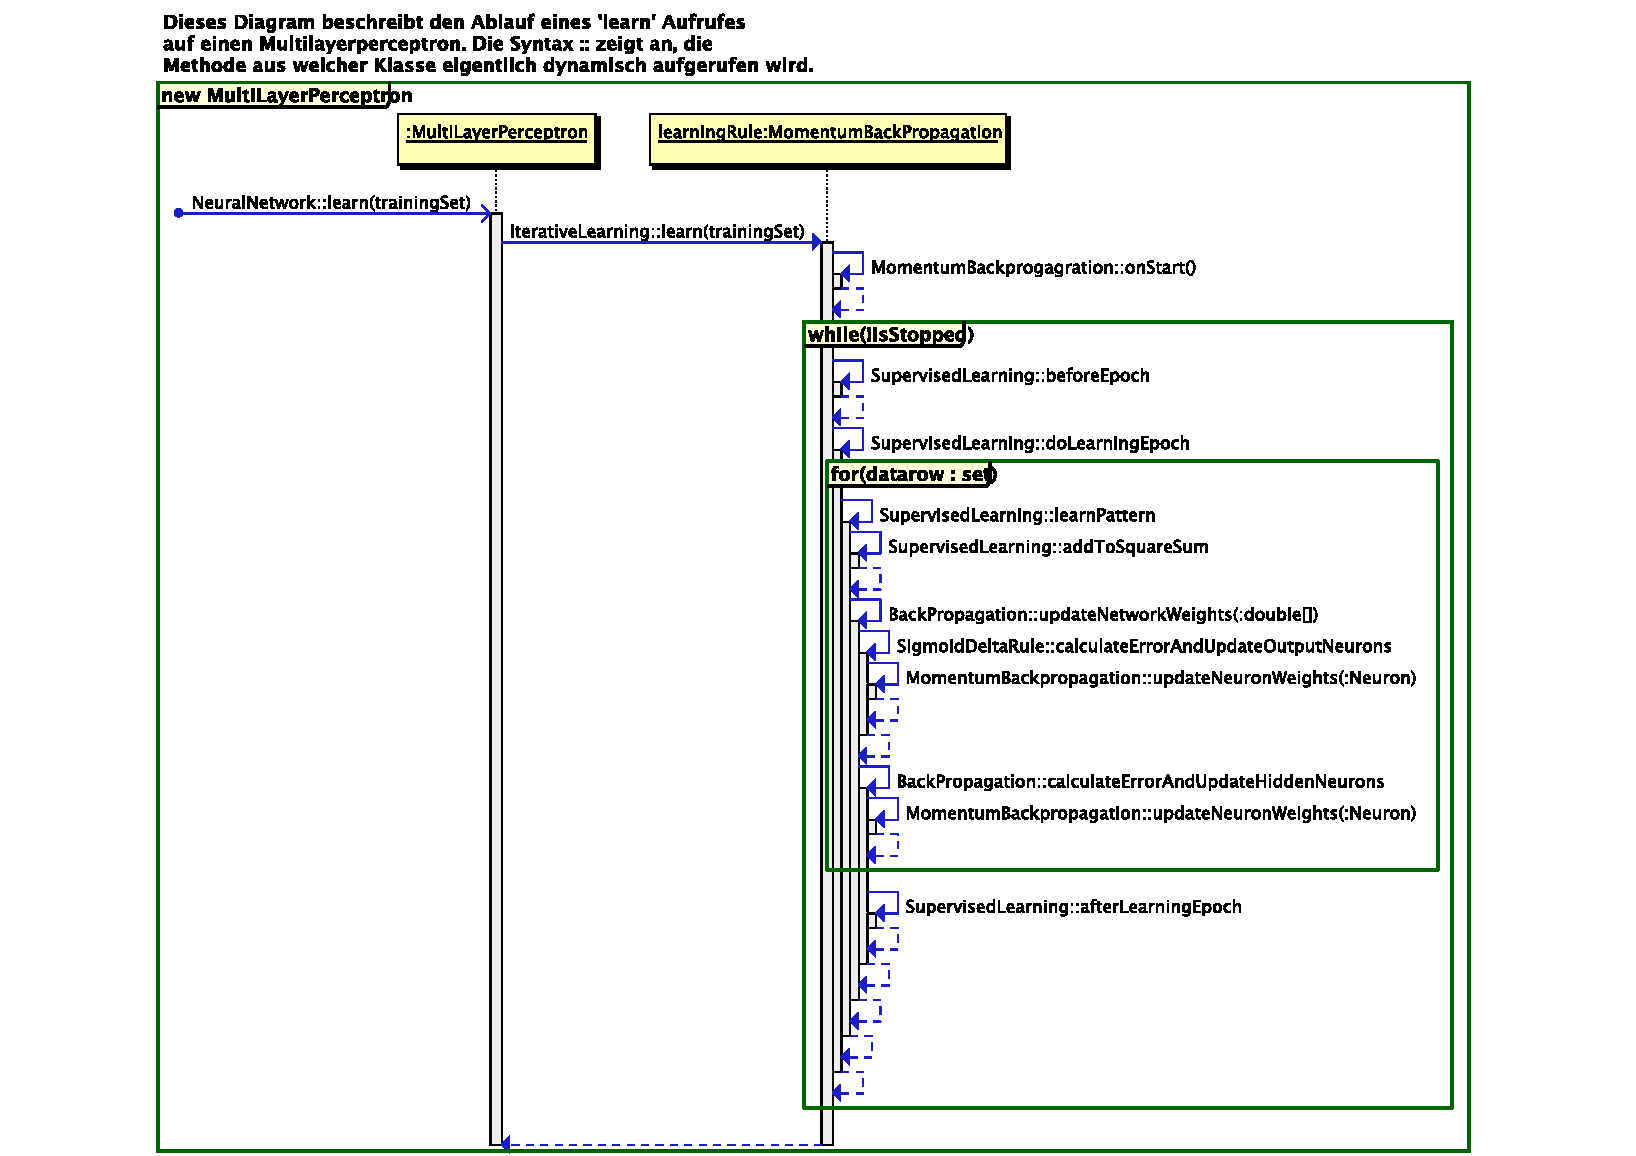
\includegraphics[scale=0.4]{images/Learn.pdf} 
			\end{center}
	\end {frame}
	
	\begin{frame}[c]\frametitle{Code Analyse \& Profiling}
		\begin{block}{Profiling}
			Methoden mit höchster akkumulierter Rechenzeit:
			\begin{itemize}
				\item $Connection.getInput()$
				\item $Connection.getWeightedInput()$
		    \end{itemize}
			$\rightarrow$ Zeit korreliert mit Anzahl der $Connections$ und Anzahl der Lern-Iterationen
		\end{block}
	\end {frame}			
	
	\begin{frame}[c]\frametitle{Parallelisierungsansätze}
		%\begin{alertblock}{}
		%\textit{TODO: Hier alle Unterpunkte rausnehmen (auf nachfolgende Seiten verteilen) und nur als kurze Übersichtsfolie nutzen??} Ja.
		%\end{alertblock}
		\begin{itemize}
			\item Layer-Partitionierung
			%\begin{itemize}
				%\item Mehrere Neuronen einer Schicht pro Thread
				%\item Langsam, da zu fein granular
			%\end{itemize}
			\item Batch Learning Parallelisierung
			%\begin{itemize}
				%\item Batch parallelisieren
				%\item Einfacherer zu parallelisieren
			%\end{itemize}
			\item Clonebased Parallelisierung
			%\begin{itemize}
				%\item Ergebnis entspricht nicht dem Orginal
				%\item Lernen bleibt unmodifiziert 
			%\end{itemize}
		\end{itemize}	
	\end{frame}
	
	\begin{frame}[c]\frametitle{Layer-Partitionierung}
		\begin{itemize}
			\item Ansatz:
			 \begin{itemize}
				\item Parallel Auswertung innerhalb partitionierter Neuronenschichten
			\end{itemize}
			\item Evaluation:
			\begin{itemize}
				\item Zu feingranular, Concurrency-Overhead überwiegt erhoffte Zeitersparnis
			\end{itemize}
		\end{itemize}	
	\end{frame}

	\begin{frame}[c]\frametitle{Batch Learning Parallelisierung}
		\begin{itemize}
			\item Batch Learning
			\begin{itemize}
				\item Summieren der Deltas (pro Verbindung)
				\item Aktualisieren erst nach einer Epoche
			\end{itemize}
			\item Ablauf:
			\begin{itemize}
				\item Aufteilen der Lerndaten
				\item Jeder Thread summiert Deltas
				\item Aktualisieren der Gewichte
			\end{itemize}
			\item Klone des NN notwendig
		\end{itemize}
	\end{frame}
	
	\begin{frame}\frametitle{Batch Learning Parallelisierung}
		\begin{enumerate}
			\item NN klonen (tiefe Kopie)
			\item Daten aufteilen
			\item \textit{parallel:} Jeder Thread lernt seine Daten
			\item \textit{parallel:} Gewichte der Klone in das Hautp-NN mergen (und in die Klone)
			\item \textit{Barriere}n
			\item Fehlerberechnung
			\item Fehler < x ? Fertig : Goto 3
		\end{enumerate}
	\end{frame}
	
	\begin{frame}\frametitle{Clonebased Parallelisierung}
		\begin{center}
			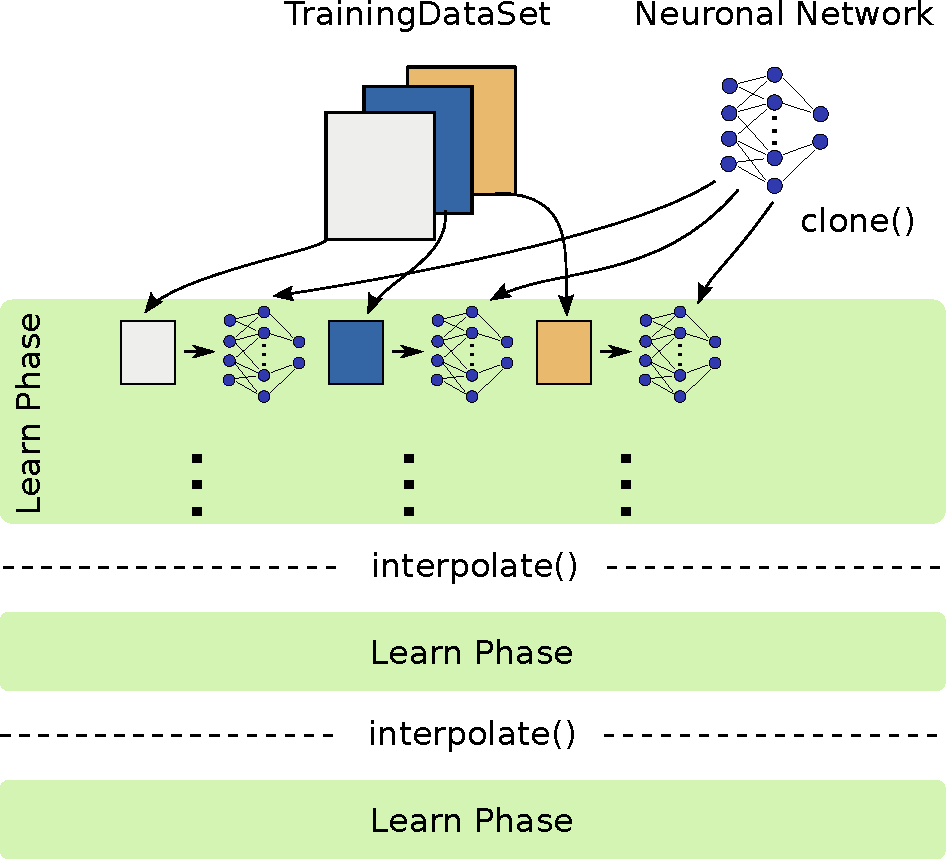
\includegraphics[width=.65\textwidth]{images/Parallelisierungsansatz.pdf} 
		\end{center}
	\end{frame}
	
	\begin{frame}\frametitle{Clonebased Parallelisierung}
		\begin{itemize}
			\item ANN wird nach der Erzeugung \glqq geklont\grqq
			\item Ein Klon pro Thread
			\item Unterschiedliche Interpolationsfunktionen
			\item Weitere Parameter
			\begin{itemize}
				\item Synchronisationsintervall
				\item Maximale Anzahl von Iterationen
			\end{itemize}				
			\item Andere Ergebnisgewichte als bei sequentiellem Lernen
			\item Wrapper für ein neuronales Netz
		\end{itemize}
	\end{frame}


	%  TODO: Dominik Clone worker parallelisierung...


%TODO: Evaluierung, Zwischenstand, Erwähnen, dass Güte über Zeit und Fehler gemessen wird. Exakt gleich Ergebnis ist nicht erforderlich. Evaluierungsframework

	\begin{frame}\frametitle{Evaluationsframework}
		\begin{block}{Score}
			wird bestimmt durch
		    \begin{itemize}
		    	\item Fehler (auf Testdaten)
		    	\item Laufzeit
		    \end{itemize}
		\end{block}
		\begin{block}{Vorgehen}
		    \begin{enumerate}
		    	\item Permutation der Daten
		    	\item Aufteilung in Trainings- und Testdaten
				\item $foreach$ ILearner L $do$
				\begin{itemize}
					\item Lerne Trainingsdaten und messe Ausführungszeiten
					\item Berechne Fehler auf Testdaten
				\end{itemize}
				\item Wiederhole ab 1 bis gewünschte Anzahl an Läufen erreicht
		    \end{enumerate}
		\end{block}
	\end{frame}
	
	\begin{frame}\frametitle{Aktuelle Evaluationswerte}
		\begin{block}{Experiment-Konfiguration}
			\begin{itemize}
				\item 5000 Datenreihen aus CERN-Satz, 1:1 Trainings-/Testdaten
				\item Intel Core2Quad Q6600, 4 Kerne à 2,4GHz, 8GB RAM
				\item JDK 7
			\end{itemize}
		\end{block}
		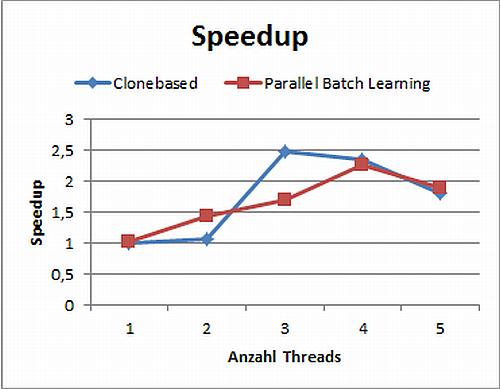
\includegraphics[width=0.51\textwidth]{images/eval_speedup.png}
		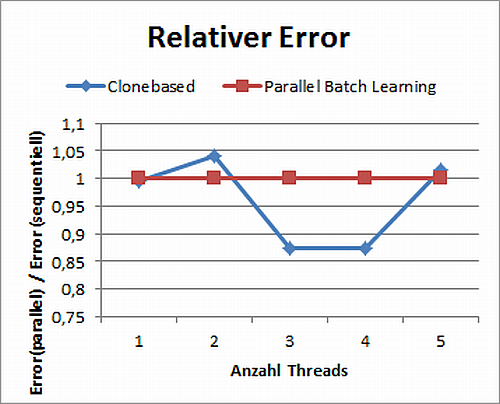
\includegraphics[width=0.49\textwidth]{images/eval_error.png}
	\end{frame}

	\begin{frame}\frametitle{Whats next?}
		\begin{block}{Fahrplan}
		    \begin{itemize}
		    	\item Vollständige Evaluierung der Ansätze
		    	\item Experimentieren mit unterschiedlichen Konfigurationsparametern $\rightarrow$ Auswirkungen auf Speedup und Error
		    \end{itemize}
		\end{block}
	\end{frame}

\end{document}